% Created 2016-05-29 Sun 18:00
\documentclass[11pt]{article}
\usepackage[utf8]{inputenc}
\usepackage[T1]{fontenc}
\usepackage{fixltx2e}
\usepackage{graphicx}
\usepackage{longtable}
\usepackage{float}
\usepackage{wrapfig}
\usepackage{rotating}
\usepackage[normalem]{ulem}
\usepackage{amsmath}
\usepackage{textcomp}
\usepackage{marvosym}
\usepackage{wasysym}
\usepackage{amssymb}
\usepackage{hyperref}
\tolerance=1000
\author{Mitch Richling}
\date{YYYY-MM-DD}
\title{DOCUMENT TITLE}
\hypersetup{
  pdfkeywords={some keywords},
  pdfsubject={},
  pdfcreator={Emacs 24.4.1 (Org mode 8.2.10)}}
\begin{document}

\maketitle
\tableofcontents


\section{Math}
\label{sec-1}

Here is some math $5+3^4$.

Here is some display math $$\sum 4$$

\section{Markup}
\label{sec-2}

\subsection{Inline stuff}
\label{sec-2-1}

Some \textbf{bold} text.

Some \emph{italics} text.

Some \uline{underlined} text.

Some \texttt{verbatim} text.

Some \verb~code~ text.

Some \sout{strike-through} text.

\subsection{Structural stuff}
\label{sec-2-2}

\subsubsection{Special Paragraphs}
\label{sec-2-2-1}

Here we have a quote:
\begin{quote}
A human being is a part of a whole, called by us \uline{universe}, a part limited in time and space. He experiences himself, his thoughts and feelings as something
separated from the rest\ldots{} a kind of optical delusion of his consciousness. This delusion is a kind of prison for us, restricting us to our personal desires
and to affection for a few persons nearest to us. Our task must be to free ourselves from this prison by widening our circle of compassion to embrace all
living creatures and the whole of nature in its beauty. -- Albert Einstein
\end{quote}

We can also keep newlines intact in an indented paragraph:
\begin{verse}
Whales Weep Not! \\
\vspace*{1em}
They say the sea is cold, but the sea contains \\
the hottest blood of all, and the wildest, the most urgent. \\
\ldots{} \\
\vspace*{1em}
\hspace*{3em}-- D.H. Lawrence \\
\end{verse}

We can have a "verbatim" section like this -- it will have the same background as the Emacs session for HTML export.
\begin{verbatim}
     Here is some text.
Note that
 everything is    just as typed.
\end{verbatim}

\subsubsection{Tables}
\label{sec-2-2-2}

\begin{center}
\begin{tabular}{l|l|rl}
\hline
col 1 & col 2 & col 3 & Col 4\\
\hline
another & bit & 1 & 2\\
a & b & 2 & 1\\
\hline
\end{tabular}
\end{center}

\subsubsection{Lists}
\label{sec-2-2-3}

Here is itemized list:

\begin{itemize}
\item first
\item second
\item third
\end{itemize}

Here is enumerated list:

\begin{enumerate}
\item First
\item Second
\item Third
\end{enumerate}

A bit of both:

\begin{enumerate}
\item First
\item Second
\begin{itemize}
\item first
\item second
\item third
\end{itemize}
\item Third
\end{enumerate}

\subsection{Todo/action items}
\label{sec-2-3}

\subsubsection{{\bfseries\sffamily TODO:NEW} This is a todo}
\label{sec-2-3-1}

\subsubsection{{\bfseries\sffamily ACTION:DONE} This is an action item -- work speak. ;)}
\label{sec-2-3-2}

\subsubsection{{\bfseries\sffamily ACTION:NEW} This is an item with sub-items [1/2]}
\label{sec-2-3-3}
\begin{enumerate}
\item {\bfseries\sffamily ACTION:DONE} A subitem
\label{sec-2-3-3-1}
\item {\bfseries\sffamily ACTION:NEW} Another subitem
\label{sec-2-3-3-2}
\end{enumerate}

\subsubsection{{\bfseries\sffamily ACTION:NEW} Here is an action item with list compoents [2/3]}
\label{sec-2-3-4}
\begin{itemize}
\item $\square$ Step 1
\item $\boxtimes$ Step 2
\item $\boxtimes$ Step 3
\end{itemize}

\section{Images}
\label{sec-3}

\subsection{PDFs in \LaTeX{} and Raster Image in HTML}
\label{sec-3-1}

In this Section you will see one image.  A PNG for HTML, and a PDF for \LaTeX{}!

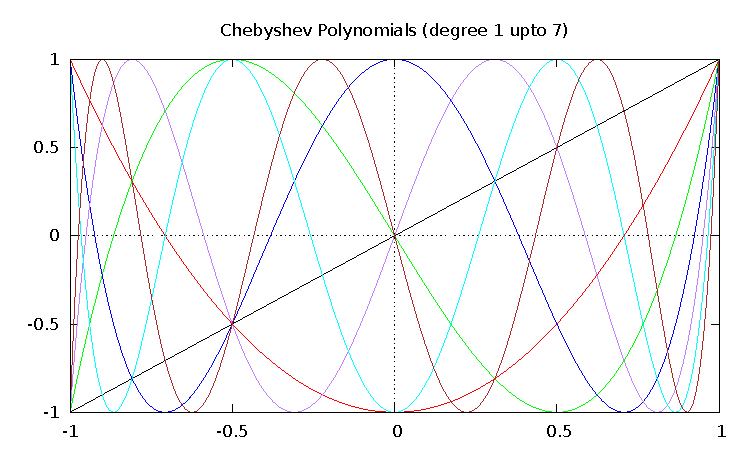
\includegraphics[width=4in]{example.pdf}

\subsection{Links to images and converting PDFs to high quality raster images}
\label{sec-3-2}

Here we have a pretty graph (in a PNG file):

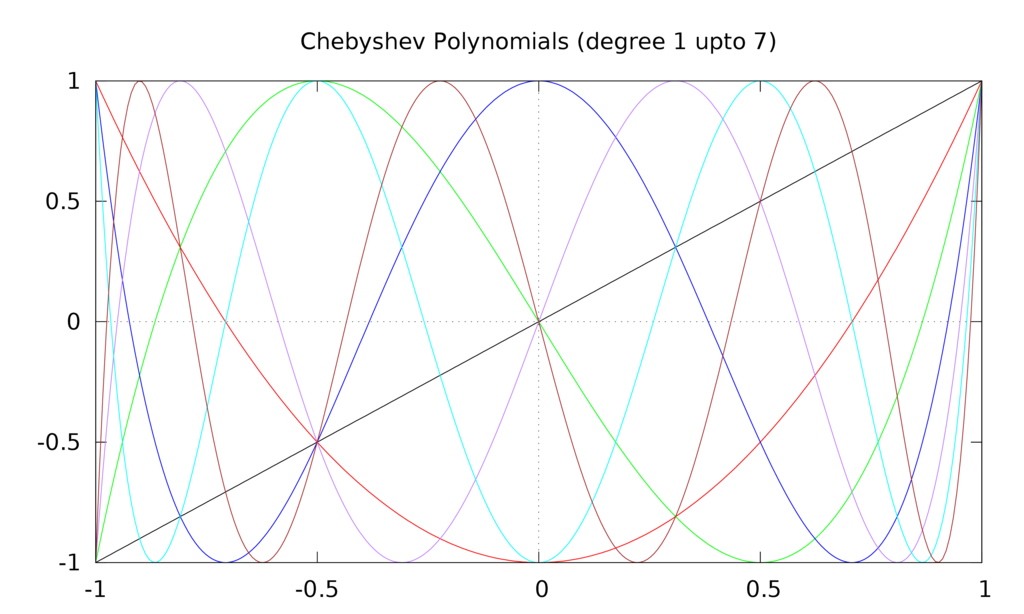
\includegraphics[width=.9\linewidth]{example.png}

The above file was generated from a high quality PDF file: \href{example.pdf}{example.pdf}. Note that the link in the previous sentence is a link in both HTML and \LaTeX{} because
the link has a 'display text' component.

The conversion was done like so:

\begin{verbatim}
convert -density 600 -resize 1024 -background white -flatten example.pdf example.png
\end{verbatim}

\section{Including external code}
\label{sec-4}

Some Ruby code is the file \url{example.rb}.  It's contents are listed below:

\begin{verbatim}
#!/usr/local/bin/ruby

##
# @file      hello.rb
# @author    Mitch Richling <http://www.mitchr.me/>
# @Copyright Copyright 2006 by Mitch Richling.  All rights reserved.
# @brief     The classic hello world program the Ruby way.@EOL
# @Keywords  ruby example hello world
# @Std       Ruby 1.8
#
#            The methods puts, print, printf & putc are all in the IO
#            class as well so that they can be used to write to
#            different IO streams.  As used here, they write to
#            STDOUT.

puts("Hello, World!")

print("Hello, World!\n")

printf("Hello, World!\n")

STDOUT << "Hello, World!\n"

STDOUT.write("Hello, World!\n")

"Hello, World!\n".each_byte {|b| putc(b) }
\end{verbatim}

\section{Inline Code}
\label{sec-5}

Here is a number, \texttt{6}, that comes from a bit of elisp code.

\section{Code Blocks}
\label{sec-6}

\begin{verbatim}
> Some Mail
>> Some More
>>> Even More
>>>> Even more
\end{verbatim}

We can use a code block just to get some highlighting!

\begin{verbatim}
> Some Mail
>> Some More
>>> Even More
>>>> Even more
\end{verbatim}

The following code exports a "value" -- not output text.

\begin{verbatim}
(+ 1 2 3 5)
\end{verbatim}

\begin{verbatim}
11
\end{verbatim}

Some sh.  Note the following code exports "text" -- the STDOUT of the command

\begin{verbatim}
date
\end{verbatim}

\begin{verbatim}
Sun May 29 13:10:45 CDT 2016
\end{verbatim}

Some Ruby

\begin{verbatim}
puts("HI MOM")
\end{verbatim}

Some Perl

\begin{verbatim}
print "HI MOM";
\end{verbatim}

Some R

\begin{verbatim}
print("HI MOM")
\end{verbatim}

\section{dot}
\label{sec-7}

Here we do not export the code, just the results -- as an image.  This results in a nice rendering.

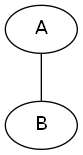
\includegraphics[width=.9\linewidth]{dotResult.png}

\section{R}
\label{sec-8}

\subsection{Run some code in a R persistent session (the someData variable is available for later blocks)}
\label{sec-8-1}
\begin{verbatim}
someData <- data.frame(a=1:10, b=rnorm(10))
print(someData)
\end{verbatim}

\subsection{Use the someData variable in the session, and draw a graph.}
\label{sec-8-2}

No speical org-mode stuff for graphics.  Just saved the output in files via R.  Add link text later.

\begin{verbatim}
g <- ggplot(someData, aes(x=a, y=b)) + geom_line()
ggsave("rOut1.png", width=8, height=6, dpi=100, units='in', plot=g);
ggsave("rOut1.pdf", width=8, height=6, dpi=600, units='in', plot=g);
\end{verbatim}

The graph:

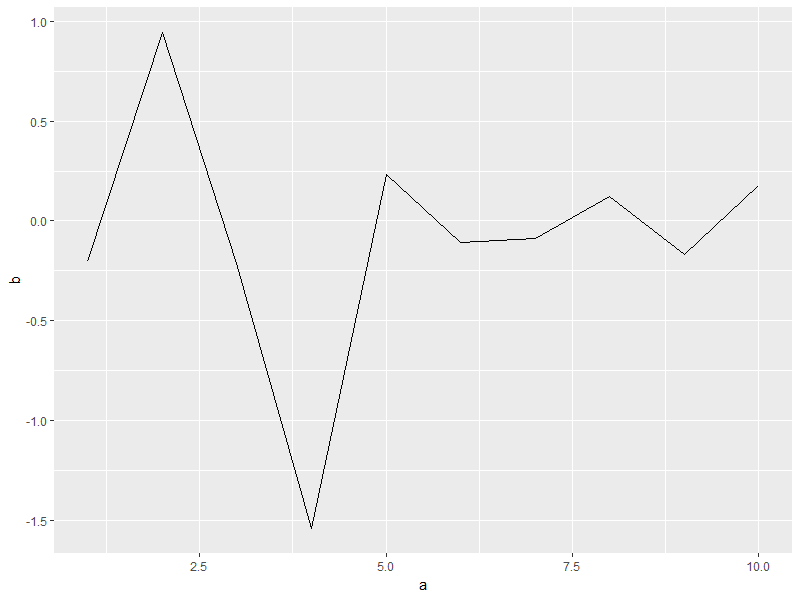
\includegraphics[width=.9\linewidth]{rOut1.png}

A high quality PDF version is \href{rOut1.pdf}{here} -- note the "here" is a link for both \LaTeX{} and HTML.

\subsection{We can use org-mode to make the file too.}
\label{sec-8-3}

Note: The graph isn't exported in HTML unless we remove the \#+RESULTS: bit.

Note: :session is required for this to work -- otherwise we must "print" the graphic.

\begin{verbatim}
ggplot(someData, aes(x=a, y=b)) + geom_line()
\end{verbatim}

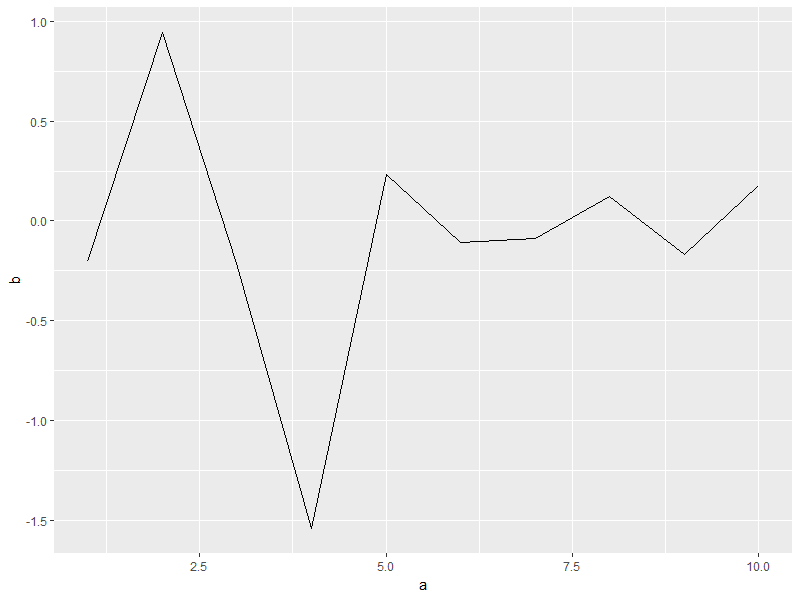
\includegraphics[width=.9\linewidth]{rOut1.png}

\section{REPRODUCIBLITY}
\label{sec-9}

This section is here to help anyone wishing to reproduce the results above, or to understand the mechanics of how the results were obtained..

\subsection{FILES}
\label{sec-9-1}

Documented in this section are (for each file in this archive):

\begin{itemize}
\item SHA1
\item Output from an 'ls -l' command
\item Output from the 'wc' command -- byte, word, and line counts
\end{itemize}

The use cases are two fold:

\begin{itemize}
\item Insure that the input data files being used are the same
\item Check if reproduced results match
\end{itemize}

Replace the \texttt{`find ./ -type f`} with a list of files and/or wildcards to explicitly select the desired files.

\begin{verbatim}
date
for c in wc 'openssl sha1' 'ls -l' ; do
    echo $c; $c `find ./ -type f`
done
\end{verbatim}

\begin{verbatim}
Sun May 29 12:54:46 CDT 2016
wc
    70     78   1236 ./auto/genericOrgTemplate.el
    13     74   3245 ./dotResult.png
   186    683  16335 ./example.pdf
  1317   7421 347721 ./example.png
    26     96    695 ./example.rb
    11     11    157 ./files_to_publish
    11     11    157 ./files_to_publish_before
  1052   4016  40754 ./genericOrgTemplate.html
   151    615   5169 ./genericOrgTemplate.html~
   530   2301  16091 ./genericOrgTemplate.org
  5096  13519 447591 ./genericOrgTemplate.pdf
   483   1302  11013 ./genericOrgTemplate.tex
    83    289   4549 ./rOut1.pdf
    58    683  18097 ./rOut1.png
   175    688  17665 ./rOut2.png
  9262  31787 930475 total
openssl sha1
SHA1(./auto/genericOrgTemplate.el)= b5365d66ab076cb63c33f86a397af8b023d9ca7f
SHA1(./dotResult.png)= af750b51add624017c0a4622c383b08589fc5a46
SHA1(./example.pdf)= 32331c8ba2289b7b3c44b494c738ef0ad9973980
SHA1(./example.png)= d193ac9077e6616ee3d849184453195c414c49c9
SHA1(./example.rb)= ee55cdae5e8017b96fe18ab376356ff6d610ab78
SHA1(./files_to_publish)= f912ac87b274c3575fe7617f4d582abb75118784
SHA1(./files_to_publish_before)= fd8a676303b873f128f526b91414889431db590a
SHA1(./genericOrgTemplate.html)= b7eeb71a8ded924cd77d1a9210afbfe256efe345
SHA1(./genericOrgTemplate.html~)= 073f08c67ffa1f9df2edb857c200a72bea2fc98a
SHA1(./genericOrgTemplate.org)= 6d7c1c0f7b11f579d9e41dd5023ba9e3ebd18e55
SHA1(./genericOrgTemplate.pdf)= 9be6c3716234ccc181e88f1f281d3480f201742e
SHA1(./genericOrgTemplate.tex)= e797b80a19d841d66fb22a25be68ef13094a8817
SHA1(./rOut1.pdf)= 4ac15c123caf08806b0ca69c0ae8a92cd884221b
SHA1(./rOut1.png)= cc8c3d82e258be1d98a6fc27d8bfa33804fa9eb3
SHA1(./rOut2.png)= 0a9b953ca71d1e25266c13ebc5e02d3825a11365
ls -l
-rw------- 1 richmit richmit   1236 Nov  2  2015 ./auto/genericOrgTemplate.el
-rw------- 1 richmit richmit   3245 Nov  1  2015 ./dotResult.png
-rw------- 1 richmit richmit  16335 May 30  2015 ./example.pdf
-rw------- 1 richmit richmit 347721 May 30  2015 ./example.png
-rw------- 1 richmit richmit    695 May 30  2015 ./example.rb
-rw------- 1 richmit richmit    157 May 29 12:31 ./files_to_publish
-rw------- 1 richmit richmit    157 May 29 12:31 ./files_to_publish_before
-rw------- 1 richmit richmit  40754 May 29 12:53 ./genericOrgTemplate.html
-rw------- 1 richmit richmit   5169 May 29 12:53 ./genericOrgTemplate.html~
-rw------- 1 richmit richmit  16091 May 29 12:52 ./genericOrgTemplate.org
-rw------- 1 richmit richmit 447591 Nov  2  2015 ./genericOrgTemplate.pdf
-rw------- 1 richmit richmit  11013 Nov  2  2015 ./genericOrgTemplate.tex
-rw------- 1 richmit richmit   4549 Nov  1  2015 ./rOut1.pdf
-rw------- 1 richmit richmit  18097 Nov  1  2015 ./rOut1.png
-rw------- 1 richmit richmit  17665 Nov  1  2015 ./rOut2.png
\end{verbatim}

\subsection{ENVIRONMENT}
\label{sec-9-2}

The input files are only part of the reproduciblity equation.  It is also important to understand the tools and computational environment used for the
original analysis.  This section contains various bits of meta-data about the tools and system I used for this analysis.

\subsubsection{Embedded Ruby Version}
\label{sec-9-2-1}

\begin{verbatim}
puts(RUBY_VERSION)
\end{verbatim}

\subsubsection{Embedded Perl Version}
\label{sec-9-2-2}

\begin{verbatim}
print $]
\end{verbatim}

\subsubsection{Embedded R Information}
\label{sec-9-2-3}

\begin{enumerate}
\item R version
\label{sec-9-2-3-1}

\begin{verbatim}
R.version
\end{verbatim}

\item Session Information
\label{sec-9-2-3-2}

\begin{verbatim}
sessionInfo()
\end{verbatim}

\item Loaded Package Versions
\label{sec-9-2-3-3}

\begin{verbatim}
installed.packages()[(loadedNamespaces()),c('Version', 'LibPath')]
\end{verbatim}
\end{enumerate}

\subsubsection{Emacs Information}
\label{sec-9-2-4}

\begin{enumerate}
\item Emacs Version
\label{sec-9-2-4-1}

\begin{verbatim}
(emacs-version)
\end{verbatim}

\item org-mode Version
\label{sec-9-2-4-2}

\begin{verbatim}
org-version
\end{verbatim}

\item ESS Version
\label{sec-9-2-4-3}

\begin{verbatim}
(ess-version)
\end{verbatim}

\item Process Environment
\label{sec-9-2-4-4}

\begin{verbatim}
process-environment
\end{verbatim}

\item System Type
\label{sec-9-2-4-5}

\begin{verbatim}
system-type
\end{verbatim}

\item System Configuration
\label{sec-9-2-4-6}

\begin{verbatim}
system-configuration
\end{verbatim}
\end{enumerate}

\subsubsection{System Information}
\label{sec-9-2-5}

\begin{verbatim}
for e in date whoami groups id hostname domainname dnsdomainname 'ifconfig -a' 'uname -a' 'openssl version' locale 'ldconfig -p' 'dpkg-query -l'; do
  c=`echo $e | awk '{print $1}'`;
  if hash $c 1>/dev/null 2>/dev/null; then 
    ruby -e 'puts("="*90)'
    echo $e
    sh -c "$e"
  fi
done
\end{verbatim}

\subsubsection{Command Line Tool Information}
\label{sec-9-2-6}

\begin{verbatim}
for e in gcc g++ gfortran                               \
         wc ls grep sed awk cut sort uniq               \
         bash ksh tcsh dash csh sh                      \
         vi vim emacs em                                \
         ruby ruby1.8 ruby2 python3 python2 perl        \
         gnuplot maxima octave M2 gap julia R           \
         qtiplot ggobi                                  \
         povray                                         \
         openscad xcircuit                              \
         convert pqiv import display                    \
         gs pdftex pdflatex tex latex dvips             \
         sbcl clisp ecl ccl                             \
         diff diff3 patch merge                         \
         sqlite3 mysqld                                 \
         paraview visit                                 \
         grass                                          \
         tar gzip bzip2 ; do
  ruby -e 'puts("="*90)'
  echo "Tool: $e"
  if hash $e 1>/dev/null 2>/dev/null; then 
    CPH=`which $e`
    if [ -n "$CPH" -a -e "$CPH" ] ; then
      echo $CPH    | sed 's/^/  Path: /'
      ls -ld $CPH  | sed 's/^/  ls-l: /'
      $e --version | sed 's/^/  Ver:  /'
    else
      echo "  Unable to locate (which): $e"
    fi
  else
    echo "  Unable to locate (hash): $e"
  fi
done
ruby -e 'puts("="*90)'
\end{verbatim}


\section{Publishing}
\label{sec-10}

By "publishing" I mean simply copying stuff from the current directory tree to a new location -- usually one shared by a web/file server or to a staging area
to be later uploaded to a web server.

To control very precicely what gets published, put the files in the file \url{files_to_publish}.  One way to do that is like so:

\begin{verbatim}
EXT2PUB='.org .html .png .gif .jpeg .pdf .ps .sh .rb .R .c .cpp .h .hpp .csv .csv.gz'
if test -e files_to_publish; then cp files_to_publish files_to_publish_before; wc -l files_to_publish_before; fi
for e in $EXT2PUB; do
  find ./ -name "*$e"
done | sed 's/^\.\///' | egrep -v '^(#|\.)' > files_to_publish
sort files_to_publish | uniq > files_to_publish~
mv files_to_publish~ files_to_publish
wc -l files_to_publish
\end{verbatim}

\begin{verbatim}
11 files_to_publish_before
11 files_to_publish
\end{verbatim}

The following will copy the current directory tree to \texttt{\$PUB\_DIR} with the modes specified by \texttt{\$PUB\_MODES} (set it to an empty string to use the modes on the
source files).  Automatically will use \texttt{files\_to\_publish} and/or \texttt{.rsync-filter} if found.  This will not publish unless the file specified by \texttt{\$HTML\_NAME} is
the newest thing in the current directory tree -- set the variable to an empty string to suppress this behavior.

\begin{verbatim}
PUB_DIR=/tmp/foo
HTML_NAME=genericOrgTemplate.html
PUB_MODES=a+rX
VERBOSE=N
if test 0 -eq `find ./ -cnewer "$HTML_NAME" -a -type f 2>/dev/null | wc -l `; then
  if test ! -e "$PUB_DIR"; then mkdir -pv "$PUB_DIR"; fi
  if test -e "$PUB_DIR"; then
    RSYNC_OPTS='--delete -a'
    if test "$VERBOSE" = "Y";      then CHMOD_OPTS="-c"; fi
    if test "$VERBOSE" = "Y";      then RSYNC_OPTS="$RSYNC_OPTS -v"; fi
    if test -e '.rsync-filter';    then RSYNC_OPTS="$RSYNC_OPTS -F"; fi
    if test -e 'files_to_publish'; then RSYNC_OPTS="$RSYNC_OPTS --files-from=files_to_publish"; fi
    rsync $RSYNC_OPTS ./ "$PUB_DIR"
    if test -n "$PUB_MODES" ; then find "$PUB_DIR" \( -type f -o -type d \) -exec chmod $CHMOD_OPTS a+rX {} \; ; fi      
    date
    echo Publish directory contains `find "$PUB_DIR" | wc -l` files consuming `du -sk "$PUB_DIR" | awk '{print $1};'`KB of space.
  else
    echo "ERROR: Unable to create target directory ($PUB_DIR)!"
  fi
else
  echo "ERROR: $HTML_NAME is not the newest file here.  Please regenerate it (C-c C-e h h)!"
fi
\end{verbatim}

\begin{verbatim}
ERROR: genericOrgTemplate.html is not the newest file here.  Please regenerate it (C-c C-e h h)!
\end{verbatim}


\section{EOF}
\label{sec-11}
% Emacs 24.4.1 (Org mode 8.2.10)
\end{document}
